 %%%%%%%%%%%%%%%%%%%%%%%%%%%%%%%%%%%%%%%%%% 
 % @File    : c:\Users\Administrator\Desktop\GNN\tutorial\sections\Graph-Structure.tex
 % @Date    : 2020-12-08 17:23:06
 % @Author  : RankFan
 % @Email   : 1917703489@qq.com
 % -----
 % Last Modified: 2020-12-14 16:03:43
 % Modified By: Rank_fan
 % -----
 %%%%%%%%%%%%%%%%%%%%%%%%%%%%%%%%%%%%%%%%%% 

\section{Graph Types \& Structures}
     在CNN中,可以将图片转换为RGB的像素矩阵,这种数据可视为时序数据,其他的时序数据还包括语音数据等类型,同时现实中也存在多种信息网络数据,社交网络、金融关系、交通流量网络包括生物学中的蛋白质分子结构,都会涉及大量的高度关联数据。这些数据构成庞大的图,图数据库就是呈现和查询这些关联的做好的方式。

     从数学定义上来说,图是{\bf 节点(vertex,或者 node) }和{\bf 边(Edge)}的集合,在一张图中,一个节点代表一个实体的特征,边,就是关联这些节点的关系 (relation) ,通常这些节点的关系我们会想办法去用数字描述。

     \begin{mydef}[Graph] 
        A graph G is a tuple  $ G = (V, E)  $ of vertices $V$ and edges $E$. For  undirected graphs, edges are subsets of cardinality two of the vertices, so each edge is of the form $(u, v)$ with $u, v \in V$. For directed graphs, the order of the edges in the tuple $(u, v) $is
        relevant to indicate the direction of the edge. If not mentioned otherwise, we will assume
        that a graph is undirected and has no self-loops, i.e. edges for which $u = v$.
     \end{mydef} 

     \begin{mydef}[Degree]
        The degree of a vertex $v$ of an undirected graph $G = (V, E)$ is the number of vertices that are connected to $v$ by means of an edge, i.e. $ deg (v) : 
        \left |  \left \{ u|\left ( u,v \right )  \in E,u \neq v \right \} \right |  $ For directed graphs, a vertex has an {\bf in-degree} and an {\bf out-degree},
        depending on the direction of the edges.
     \end{mydef}

     A graph G = (V, E) may also contain labels or attributes, for example in the form of node labels, edge labels, or edge weights. This is known as an attributed graph.

     \begin{mydef}[Attributed graph]
        {\rm{An attributed graph}} is a graph that has either labels or attributes on the nodes and/or edges. When present, labels are each assumed to be defined
        over a common alphabet, $ \sum_V $ for nodes and $\sum_E$ for edges, with a function, $I_V$ for nodes and $I_E$ for edges, to assign each entity its label. We thus have 
        
        \begin{equation}
            \textstyle 
            \begin{split}
                I_{V} : V \longrightarrow \textstyle  \sum_{V} \\
                I_{E} : E \longrightarrow \textstyle  \sum_{E} 
            \end{split}
        \end{equation}

        and both of these functions need to be total. A graph with additional attributes for verticesand or edges has attribute functions
        \begin{equation}
            \textstyle 
            \begin{split}
                \mathcal{A_{V}}  : V \longrightarrow \textstyle  \mathbb{R}^{d} \\
                \mathcal{A_{V}} : E \longrightarrow \textstyle  \mathbb{  R } ^{d} 
            \end{split}
        \end{equation}

        that are typically assumed to be real-valued, i.e. d = 1. Scalar-valued edge attributes areoften also referred to as weights, with the tacit assumption that the values refer to the strength of a specific connection.

        Since a graph defines a connectivity for each of its vertices, its edges induce sequence. for visiting them. These sequences have specific names, depending on their properties.
     \end{mydef}

     \begin{mydef}[Walks, paths, and cycles]
        A sequence of k nodes  $ v_1 , v_2 , \cdots , v_k $ of the vertices of a graph G is called a walk of length k − 1 if the edge between two consecutive vertices exists.
        Vertices of a walk are allowed to repeat. 
        If, however, node repetition is not allowed, one typically refers to the node sequence as a path, the
        adjective directed often being added in the case of directed graphs. 
        Special consideration is given to cycles, i.e. walks of length k − 1 for which $v_1 = v_k$ .
     \end{mydef}

     \begin{mydef}[Random walks]
        A walk in a graph is referred to as a random walk if the next vertex (or edge) is picked in a probabilistic manner. 
        Having picked a start node at random,a typical choice, for example, would be to pick any outgoing edge of the node with uniform
        probability (in case of unweighted graphs), or with a probability proportional to its weight.
     \end{mydef}

     \begin{mydef}[Connected graph]
        A graph is said to be connected if a walk between all pairs of nodes exists. 
        \begin{myRemark}
            Specifically, in a fully connected graph, each pair of nodes is connected by an edge. If a graph is not connected, the set of its nodes can be partitioned using an equivalence relation u ~ v if and only if a walk between u and v exists. The equivalence classes under this relation are called connected components.

            Likewise, paths can also be used to assess distances in a graph. This viewpoint is oftenhelpful when approximating high-dimensional manifolds through graphs, and it is possible to give bounds on the dissimilarity of graph-based distances and geodesic distances of the manifold .
        \end{myRemark}
     \end{mydef}

     \begin{mydef}[Shortest paths and distances]
        Given two vertices u and v of a graph that are in the same connected component, among all the paths connecting them, there is at least one shortest path that has the minimum number of vertices out of all other paths connecting the two vertices.
     \end{mydef}

     \begin{mydef}[k-hop neighbourhood of a vertex]
        Given a vertex v of a graph G and $ k \in \mathbb{N}_{>0} $ its k-hop neighbourhood  $N^{(k)} (v)$ is defined as all the vertices in G that are reachable
        in at most k steps, which includes v, assuming uniform edge weights.   For example, $N^{(1)} (v)$ is just the set of vertices that are connected to v by an edge and v.
        \begin{myRemark}
            This definition can be connected to the idea of a “ball” in metric spaces by observing that each k-hop neighbourhood of a vertex v induces a subgraph of the original graph G. For increasing values of k, these induced subgraphs are nested—and for k sufficiently large, the original graph G is obtained. This concept will play an important role later on when we define graph kernels that operate at multiple scales,
        \end{myRemark}
     \end{mydef}

     \begin{mydef}[Adjacency matrix A]
        A graph is often represented through its adjacencymatrix A. A graph with n vertices will thus be represented by an n × n binary matrix whose entry Aij = 1 if the ith and jth vertex of the graph are connected by an edge. 
        \begin{myRemark}
            The adjacency matrix is symmetrical for undirected graphs, whereas for directed graphs $A_{ij}$ and $A_{ji}$ can be different depending on the edge structure. Furthermore, if edge weights are available,
            i.e. $\mathcal{A_{E} (\cdot)} $ exists and d = 1, it is also possible to derive a weighted variant of the adjacency
            matrix by setting Aij to the corresponding edge weight.
        \end{myRemark}
     \end{mydef}
     
     \begin{mydef}[Graph Laplacian]
        Let A be the adjacency matrix of a graph G = (V, E).If weights are available, each entry Aij thus consists of the weight of the corresponding edge. Furthermore, let D be the degree matrix of G. This diagonal matrix contains the degree of each vertex $v \in  V $in the unweighted case.  For weighted graphs, each entry consists of the sum of all edge weights of all edges that are incident on the corresponding vertex.Laplacian ,matrix will be a symmetric positive semi-definite matrix for undirected graphs. 
        
        \begin{equation}
            L := D − A
        \end{equation}
     \end{mydef}
\begin{figure}[ht!]
    \centering
    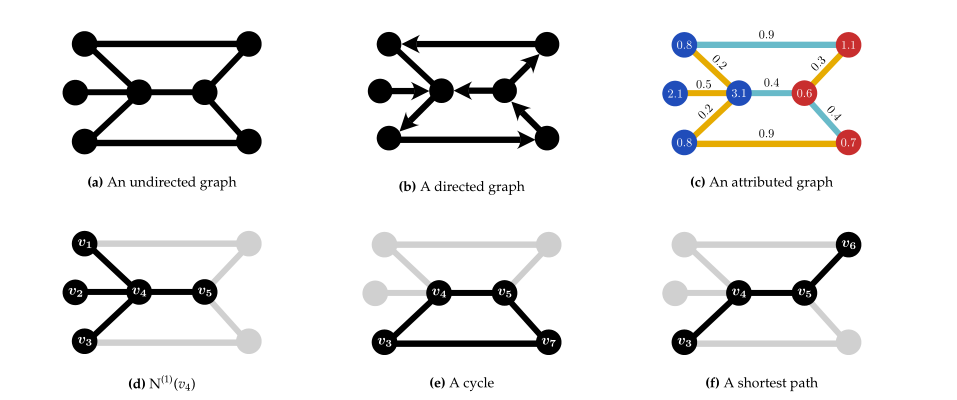
\includegraphics[scale = 0.5]{def_graph.png}
\end{figure}
\begin{figure}[htb!]
    \centering
    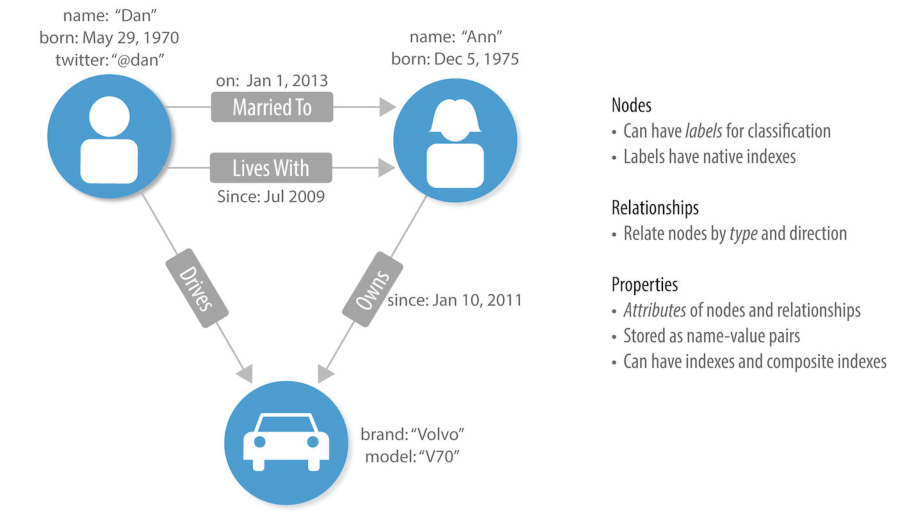
\includegraphics[scale = 0.5]{label_property.png}
    \caption{属性图}
\end{figure}